
\chapter{Theorem~1: OASG Existence}
\label{ch:theorem-oasg}

This chapter proves the \emph{Observed-safe / Actually-unsafe State Gap}
(OASG) existence theorem in the battery domain.  The theorem
establishes that telemetry degradation creates episodes where an action
is safe according to the observed state but unsafe according to the
true state---the foundational phenomenon that motivates the entire
ORIUS safety layer.

\section{Domain-Agnostic Statement}

We first state the OASG existence result for an arbitrary cyber-physical
system; the battery domain provides the concrete instantiation that follows.

\begin{definition}[Abstract CPS]
\label{def:abstract-cps}
A cyber-physical system is a tuple
$(\mathcal{X}, \mathcal{U}, f, \mathcal{S}, \hat{x})$ where
$\mathcal{X} \subseteq \mathbb{R}^n$ is the state space,
$\mathcal{U} \subseteq \mathbb{R}^m$ is the action space,
$f : \mathcal{X} \times \mathcal{U} \to \mathcal{X}$ is the (possibly
stochastic) dynamics, $\mathcal{S} \subseteq \mathcal{X}$ is the safe
set with non-empty boundary $\partial \mathcal{S} \neq \emptyset$, and
$\hat{x}_t = x_t + \xi_t$ is the observed state under telemetry error
$\xi_t$ with $\|\xi_t\| \le g(w_t)$ (Assumption~A2).
\end{definition}

\begin{theorem}[OASG Existence --- General CPS]
\label{thm:oasg-general}
Let $(\mathcal{X}, \mathcal{U}, f, \mathcal{S}, \hat{x})$ be a CPS
satisfying Assumptions A1 (bounded dynamics error), A2 (bounded telemetry
error with $g(w_t) > 0$ under degraded quality), and A4 (known dynamics).
Let $\pi : \mathcal{X} \to \mathcal{U}$ be any quality-ignorant controller,
i.e.\ one whose action depends only on $\hat{x}_t$ and not on $w_t$.

If the controller drives the state within distance
$\delta > 0$ of $\partial \mathcal{S}$ with positive frequency, and the
telemetry error satisfies $\Pr[\|\xi_t\| > \delta] > 0$, then there
exists a time $t^*$ such that
\[
  \phi_{\text{obs}}(\pi(\hat{x}_{t^*})) = 1
  \quad\text{and}\quad
  \phi_{\text{true}}(\pi(\hat{x}_{t^*})) = 0,
\]
where $\phi_{\text{obs}}$ and $\phi_{\text{true}}$ are the observed-safe
and truly-safe predicates respectively.
\end{theorem}

The proof constructs the witness $t^*$ by intersecting the boundary-proximity
set (from optimal control) with the observation-error tail (from degraded
telemetry).  We now instantiate this in the battery domain.

\section{Battery-Domain Instantiation}
\label{sec:battery-setup}

Consider a battery energy storage system with:
\begin{itemize}
  \item True state $x_t = \text{SOC}_t \in [0, E_{\max}]$ (MWh).
  \item Observed state $\hat{x}_t = x_t + \xi_t$, where $\xi_t$ is
    the telemetry error induced by packet dropout, delay, drift, or
    stale sensors.
  \item Action $a_t = (P_t^{\text{chg}}, P_t^{\text{dis}}) \in \mathbb{R}_+^2$
    subject to power and ramp constraints.
  \item Dynamics: $x_{t+1} = x_t + (\eta_c\,P_t^{\text{chg}} -
    \eta_d^{-1}\,P_t^{\text{dis}})\,\Delta t + \epsilon_t$, where
    $|\epsilon_t| \le \epsilon_{\text{model}}$ (Assumption~A1).
\end{itemize}

\section{Observed and True Safety Predicates}

\begin{definition}[Observed safety]
\label{def:obs-safe}
An action $a_t$ is \emph{observed-safe} if the predicted next state
under the observed SOC satisfies the constraints:
\[
  \phi_{\text{obs}}(a_t) \;=\; \mathbf{1}\!\bigl[\,
    \text{SOC}_{\min} \;\le\; \hat{x}_t + \Delta(a_t) \;\le\;
    \text{SOC}_{\max}\,\bigr],
\]
where $\Delta(a_t) = (\eta_c P_t^{\text{chg}} -
\eta_d^{-1} P_t^{\text{dis}})\,\Delta t$.
\end{definition}

\begin{definition}[True safety]
\label{def:true-safe}
An action $a_t$ is \emph{truly safe} if the actual next state satisfies
the constraints:
\[
  \phi_{\text{true}}(a_t) \;=\; \mathbf{1}\!\bigl[\,
    \text{SOC}_{\min} \;\le\; x_t + \Delta(a_t) + \epsilon_t \;\le\;
    \text{SOC}_{\max}\,\bigr].
\]
\end{definition}

The OASG phenomenon occurs when $\phi_{\text{obs}}(a_t) = 1$ but
$\phi_{\text{true}}(a_t) = 0$.

\section{Assumptions Used}

The OASG existence theorem requires:
\begin{itemize}
  \item \textbf{A1} (bounded model error): ensures the dynamics are
    predictable up to $\epsilon_{\text{model}}$.
  \item \textbf{A2} (bounded telemetry error): ensures the observation
    gap $|\xi_t| \le g(w_t)$ is finite but non-zero under degraded
    telemetry.
  \item \textbf{A4} (known dynamics): ensures the controller can compute
    $\Delta(a_t)$ correctly.
\end{itemize}

\section{Auxiliary Lemmas}

\begin{lemma}[Observation gap under dropout]
\label{lem:obs-gap-dropout}
Under packet dropout with rate $d > 0$, the observation error satisfies
\[
  \mathbb{E}\bigl[|\xi_t|\bigr] \;\ge\; d \cdot \sigma_{\text{drift}} \cdot
  \sqrt{\Delta t},
\]
where $\sigma_{\text{drift}}$ is the standard deviation of the one-step
state drift.
\end{lemma}

\begin{proof}
When a packet is dropped (probability $d$), the observer uses the last
received state, which drifts by at least $\sigma_{\text{drift}}\sqrt{\Delta t}$
in expectation under the sub-Gaussian drift model.  The result follows
by the law of total expectation.
\end{proof}

\begin{lemma}[Boundary proximity under arbitrage]
\label{lem:boundary-proximity}
An optimal arbitrage controller drives SOC within
$\delta_{\text{bnd}} = P_{\max}\,\Delta t$ of at least one constraint
bound in at least a fraction $f_{\text{bnd}} > 0$ of time steps.
\end{lemma}

\begin{proof}
Optimal arbitrage charges to near-full when prices are low and discharges
to near-empty when prices are high.  The fraction $f_{\text{bnd}}$
depends on the price distribution and is strictly positive whenever
price variance is non-zero.
\end{proof}

\section{Main Theorem: OASG Existence}

\begin{theorem}[OASG Existence]
\label{thm:oasg-existence}
Under Assumptions A1, A2, and A4, for any dropout rate $d > 0$ and any
optimal arbitrage controller, there exists a time step $t^*$ such that
\[
  \phi_{\text{obs}}(a_{t^*}) = 1 \quad\text{and}\quad
  \phi_{\text{true}}(a_{t^*}) = 0.
\]
That is, the controller selects an action that appears safe in the
observed state but violates a constraint in the true state.
\end{theorem}

\begin{proof}
By Lemma~\ref{lem:boundary-proximity}, there exists a set
$\mathcal{T}_{\text{bnd}} \subset \{1, \ldots, T\}$ with
$|\mathcal{T}_{\text{bnd}}| \ge f_{\text{bnd}}\,T$ such that for
$t \in \mathcal{T}_{\text{bnd}}$, the true SOC is within
$\delta_{\text{bnd}}$ of a constraint bound.

By Lemma~\ref{lem:obs-gap-dropout}, for dropout rate $d > 0$ the
observation error has $\mathbb{E}[|\xi_t|] > 0$.  In particular,
with positive probability, $|\xi_t| > \delta_{\text{bnd}}$ for
some $t \in \mathcal{T}_{\text{bnd}}$.

At such a step $t^*$, the observed state $\hat{x}_{t^*} = x_{t^*} + \xi_{t^*}$
is displaced from the true state by more than the distance to the
constraint boundary.  The controller, which sees only $\hat{x}_{t^*}$,
selects an action that is feasible under the observed state but pushes
the true state across the bound:
\[
  x_{t^*} + \Delta(a_{t^*}) < \text{SOC}_{\min}
  \quad\text{while}\quad
  \hat{x}_{t^*} + \Delta(a_{t^*}) \ge \text{SOC}_{\min}.
\]
Hence $\phi_{\text{obs}}(a_{t^*}) = 1$ and $\phi_{\text{true}}(a_{t^*}) = 0$.
\end{proof}

\section{Interpretive Table}

Table~\ref{tab:oasg-interpretation} maps the theorem's formal elements
to battery observables.

\begin{table}[ht]
\centering
\caption{Mapping OASG Existence theorem to battery domain.}
\label{tab:oasg-interpretation}
\begin{tabular}{ll}
\toprule
\textbf{Formal element} & \textbf{Battery meaning} \\
\midrule
$x_t$ & True SOC (MWh) \\
$\hat{x}_t$ & BMS-reported SOC after telemetry degradation \\
$\xi_t$ & Telemetry error from dropout / drift / delay \\
$\phi_{\text{obs}} = 1, \phi_{\text{true}} = 0$ & Controller thinks SOC is in bounds; it is not \\
$\delta_{\text{bnd}}$ & Distance from SOC to nearest rated limit \\
\bottomrule
\end{tabular}
\end{table}

\section{Artifact-Backed Figure}

Figure~\ref{fig:oasg-evidence} shows the empirical OASG rate (TSVR)
as a function of dropout rate for the deterministic LP controller.

\begin{figure}[ht]
\centering
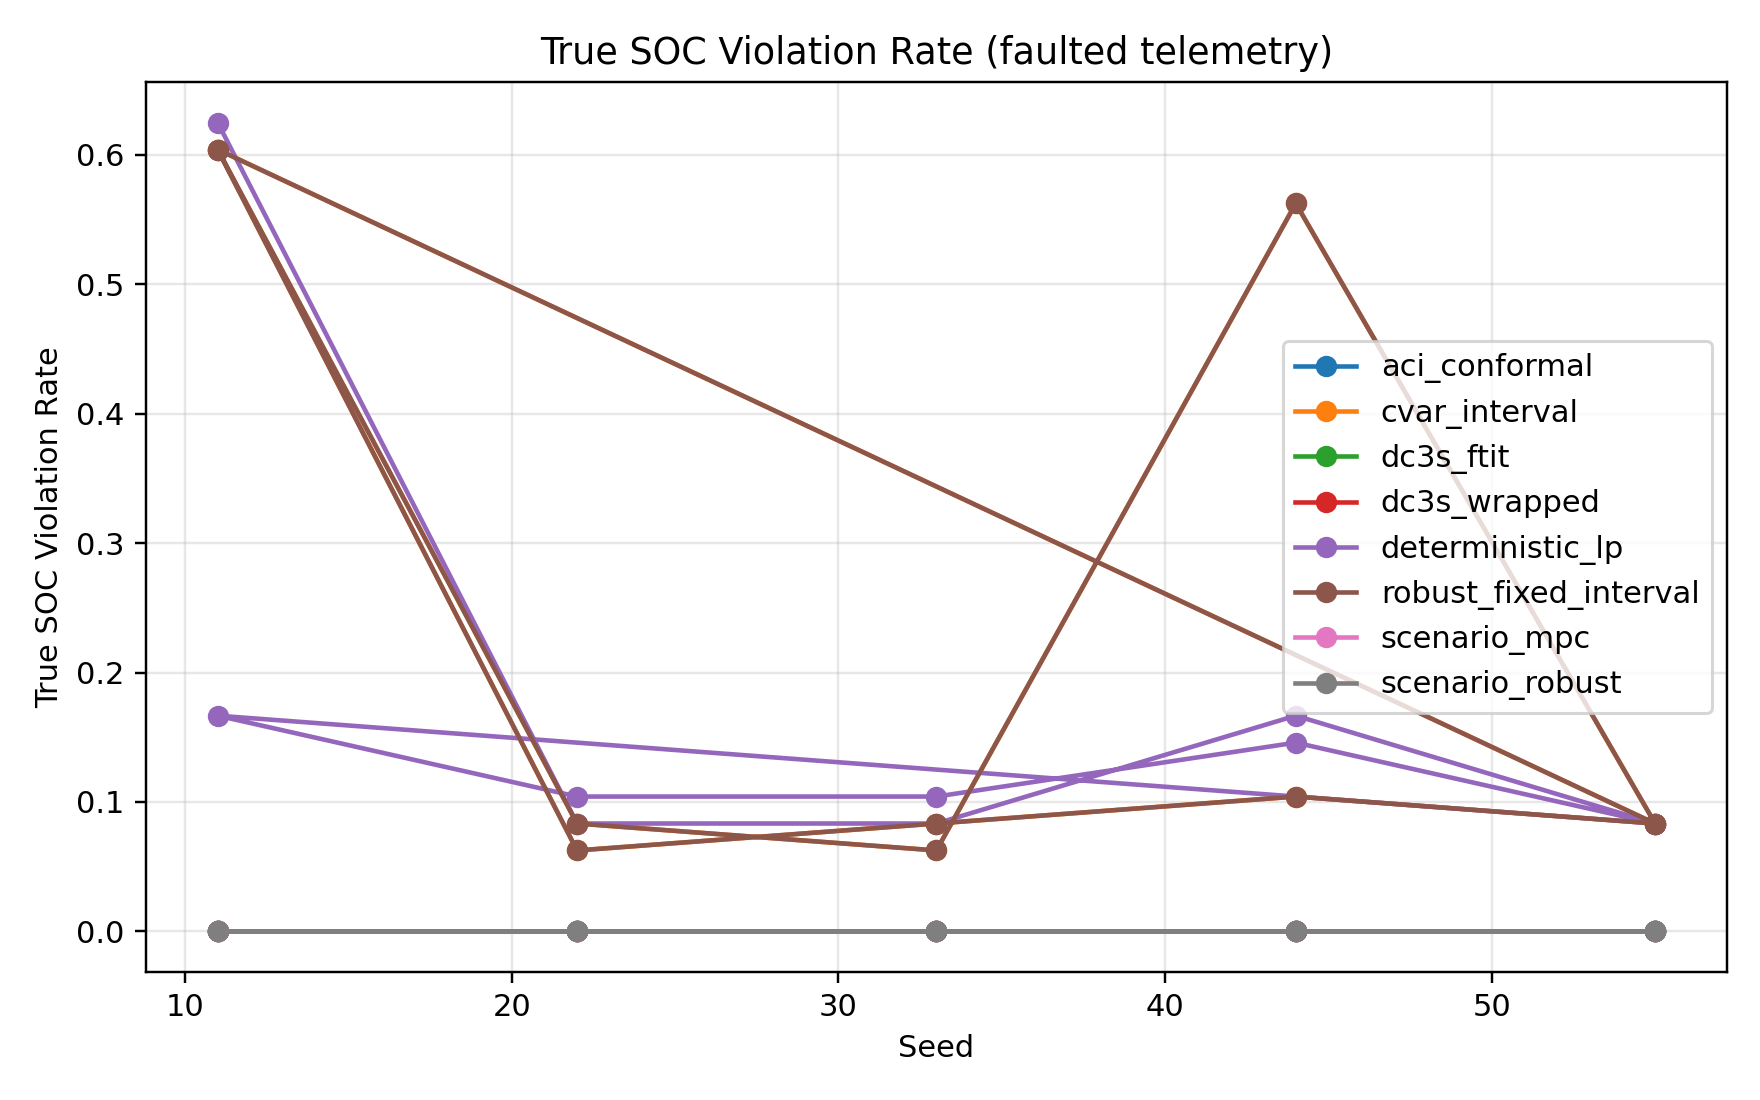
\includegraphics[width=0.85\textwidth]{paper/assets/figures/fig03_true_soc_violation_vs_dropout.png}
\caption{Empirical OASG rate (TSVR) versus dropout rate for the
  deterministic LP.  Non-zero TSVR at all $d > 0$ confirms
  Theorem~\ref{thm:oasg-existence}.}
\label{fig:oasg-evidence}
\end{figure}

\section{Corollaries}

\begin{corollary}[OASG rate lower bound]
\label{cor:oasg-rate}
Under the conditions of Theorem~\ref{thm:oasg-existence}, the expected
OASG rate satisfies
$\mathbb{E}[\text{TSVR}] \ge d \cdot f_{\text{bnd}} \cdot
\Pr[|\xi_t| > \delta_{\text{bnd}}] > 0$.
\end{corollary}

\begin{corollary}[OASG severity]
\label{cor:oasg-severity}
The expected severity of an OASG violation is at least
$\mathbb{E}[|\xi_t| - \delta_{\text{bnd}} \mid |\xi_t| > \delta_{\text{bnd}}] > 0$.
\end{corollary}

\section{What This Theorem Does Not Prove}

\begin{enumerate}
  \item It does not quantify the \emph{exact} TSVR for a specific
    controller; that requires empirical measurement (Chapter~\ref{ch:main-results}).
  \item It does not claim that \emph{every} step has a violation, only
    that at least one exists.
  \item It does not address whether the violation can be prevented---that
    is the subject of Theorem~\ref{thm:safety-preservation}.
\end{enumerate}

\section{Chapter Summary}

The OASG Existence theorem is the first rung of the theorem ladder.
It proves that the gap between observed and true safety is not a
theoretical curiosity but an inevitable consequence of telemetry
degradation in optimising controllers.  The battery domain provides
a concrete witness: a TSVR of 3.9\% for the deterministic LP under
\texttt{drift\_combo} at 20\% dropout.

%% Shared domain-instantiation block — \input{} at the end of theorem chapters.
%% It maps theorem objects only to the active Battery + AV + Healthcare claim
%% surface used by the current public manuscript.

\providecommand{\domainblockid}{generic}
\providecommand{\domainblocktitle}{\domainblockid}

\subsection{Domain Instantiation Across the Active Three-Domain Surface}
\label{sec:domain-instantiation-\domainblockid}

The theorem above is stated for an abstract CPS with observation vector
$z_t$, reliability score $w_t$, state uncertainty region
$C_t^{\text{RAC}}$, feasible action set $\mathcal{A}_t$, and violation
predicate $v(\cdot)$.  Table~\ref{tab:domain-instantiation-\domainblockid}
maps these objects to the three active public rows.  Battery is the witness
row; AV and Healthcare are bounded promoted rows with narrower evidence tiers.

\begin{table}[htbp]
\centering
\small
\caption{Domain-specific instantiation for Theorem~\domainblocktitle{} across the active three-domain surface.}
\label{tab:domain-instantiation-\domainblockid}
\begin{tabular}{p{2.6cm}p{3.3cm}p{3.3cm}p{3.3cm}}
\toprule
\textbf{Object} & \textbf{Battery} & \textbf{AV} & \textbf{Healthcare} \\
\midrule
$z_t$ (observation)
  & SCADA packet: SOC, voltage, current, load
  & nuPlan replay state: ego speed, relative gap, local context
  & ICU monitoring state: vital-sign and alert context \\
\addlinespace
$w_t$ (reliability)
  & OQE composite score over dropout, delay, stale telemetry
  & OQE score over delay, dropout, stale, out-of-order, and spike faults
  & OQE score over stale and spike degradation in retrospective monitoring \\
\addlinespace
$C_t^{\text{RAC}}$ (uncertainty region)
  & Conformal SOC interval $[\hat{s}_{\text{lo}},\hat{s}_{\text{hi}}]$
  & Conformal ego-speed and relative-gap intervals
  & Conformal vital-sign interval for alert-release monitoring \\
\addlinespace
$\mathcal{A}_t$ (feasible set)
  & Dispatch command constrained by SOC and reserve bounds
  & Longitudinal action constrained by TTC and predictive-entry barrier
  & Alert or hold decision constrained by bounded intervention discipline \\
\addlinespace
$v(\cdot)$ (violation)
  & SOC or dispatch envelope violation on true state
  & Replay-level TTC or entry-barrier violation on true state
  & Bounded monitoring or alert-release violation on retrospective trace \\
\bottomrule
\end{tabular}
\end{table}

